% elementos pré-textuais 

% título do sumário
\ifdefined\contentsname
  \renewcommand*\contentsname{SUMÁRIO}
\else
  \newcommand\contentsname{SUMÁRIO}
\fi

% capa 
% \imprimircapa

% folha de rosto 
% o * indica que haverá a ficha bibliográfica 
\imprimirfolhaderosto*

% ficha catalográfica 
% \begin{fichacatalografica}
%    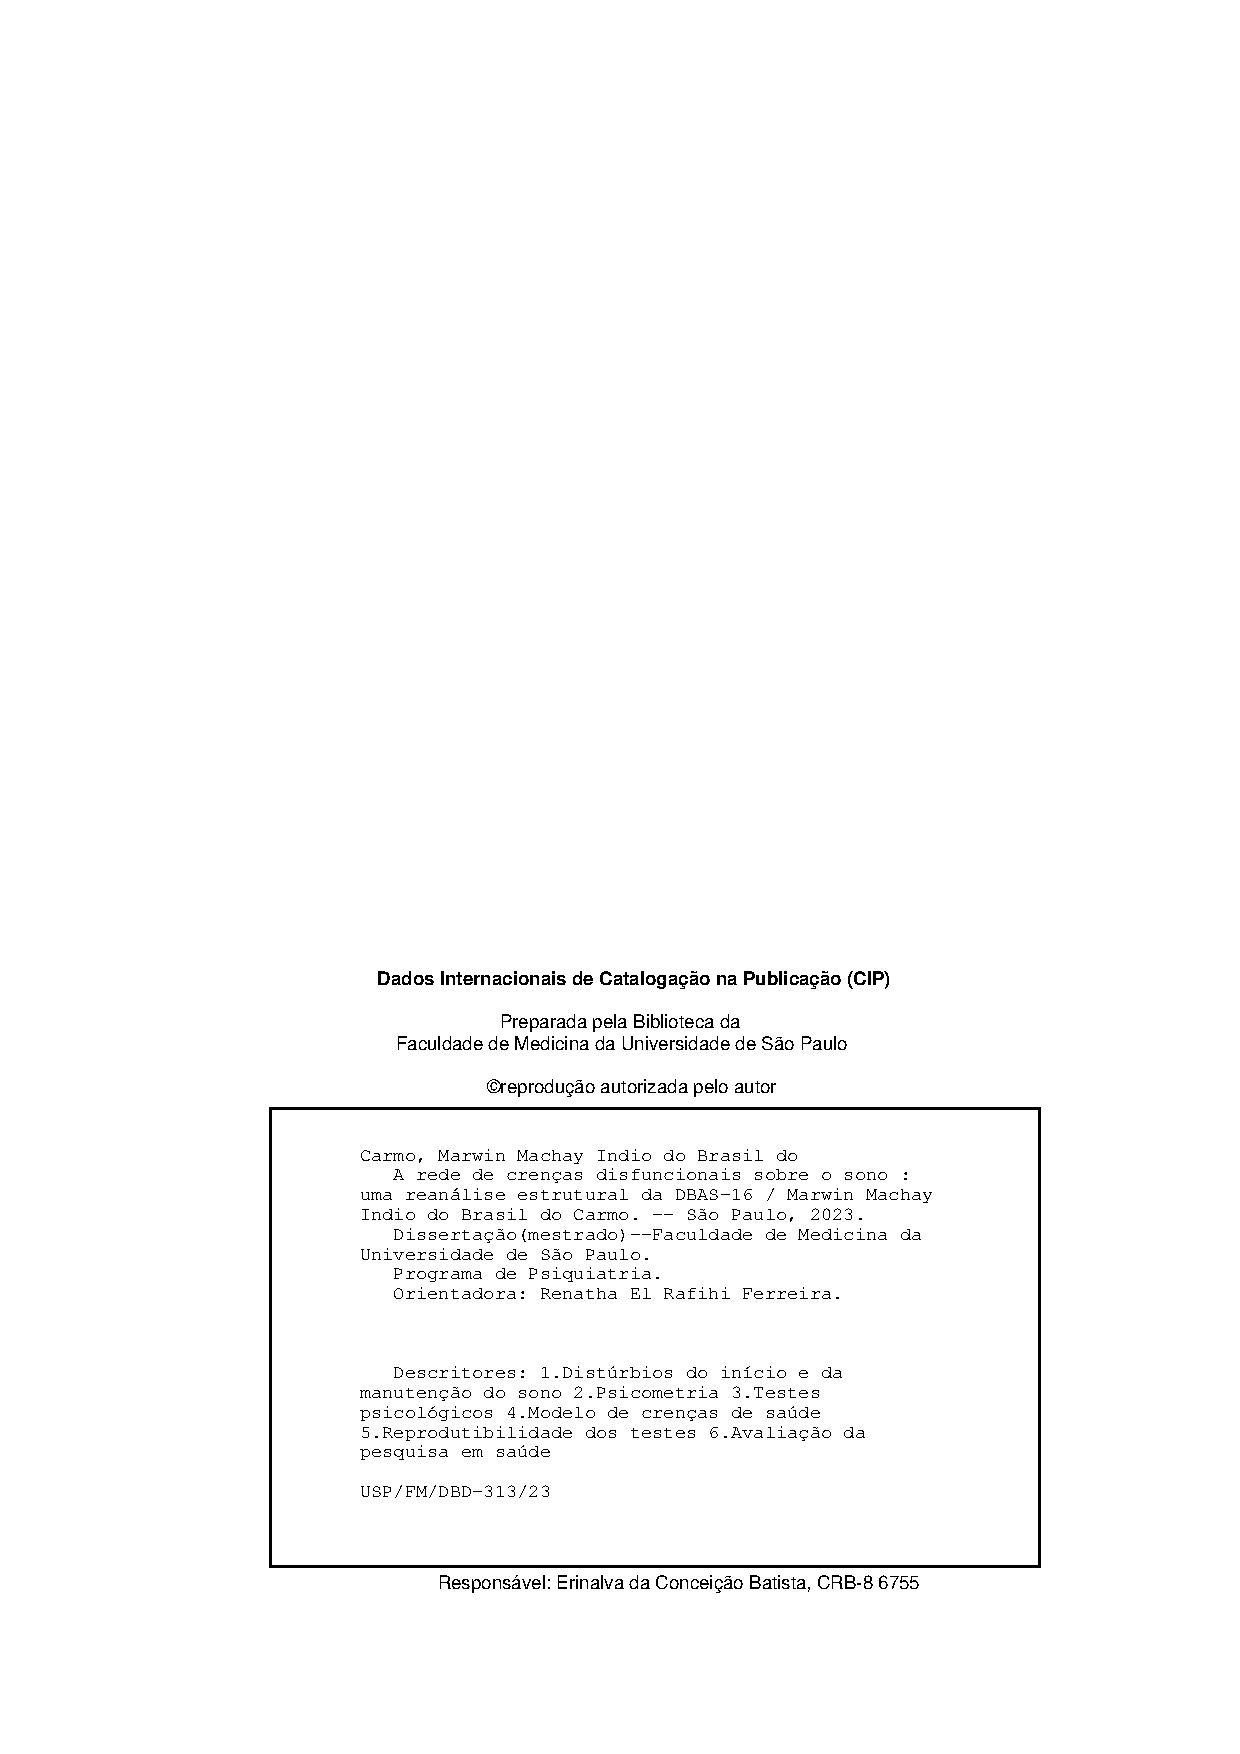
\includepdf[pages={1}]{ficha-catalog.pdf}
% \end{fichacatalografica}


% substituir pela ficha em pdf fornecida pela UFES após defesa 
\begin{fichacatalografica}
	\sffamily
	\vspace*{\fill}					% Posição vertical
	\begin{center}					% Minipage Centralizado
	\fbox{\begin{minipage}[c][8cm]{15cm}		% Largura
	\small
	\imprimirautor

	\hspace{0.5cm} \imprimirtitulo  / \imprimirautor. --
	\imprimirlocal, \imprimirdata-

	\hspace{0.5cm} \thelastpage p. : il. (algumas color.) ; 30 cm.\\

	\hspace{0.5cm} \imprimirorientadorRotulo~\imprimirorientador\\

	\hspace{0.5cm}
	\parbox[t]{\textwidth}{\imprimirtipotrabalho~--~\imprimirinstituicao,
	\imprimirdata.}\\

	\hspace{0.5cm}
		1. Palavra-chave1.
		2. Palavra-chave2.
		2. Palavra-chave3.
		I. Orientador.
		II. Universidade xxx.
		III. Faculdade de xxx.
		IV. Título
	\end{minipage}}
	\end{center}
\end{fichacatalografica}

% folha de aprovação 
%
%\begin{folhadeaprovacao}
%    \includepdf{folhadeaprovacao_final.pdf}
%\end{folhadeaprovacao}


% substituir pela folha assinada pela banca após defesa 
\begin{folhadeaprovacao}

  \begin{center}
    {\ABNTEXchapterfont\large\imprimirautor}

    \vspace*{\fill}\vspace*{\fill}
    \begin{center}
      \ABNTEXchapterfont\bfseries\Large\imprimirtitulo
    \end{center}
    \vspace*{\fill}
    
    \hspace{.45\textwidth}
    \begin{minipage}{.5\textwidth}
        \imprimirpreambulo
        \vspace*{1cm}
        Trabalho aprovado em:\\[2cm]
        \textbf{Banca Examinadora} \\
        \assinatura{\textbf{\imprimirorientador} \\ Universidade de São Paulo \\ Orientadora} 
        \assinatura{\textbf{Dra. Ila Marques Porto Linares} \\ Universidade Federal De São Paulo}
        \assinatura{\textbf{Dr. Altay Alves Lino de Souza} \\ Universidade Federal De São Paulo}
        %\assinatura{\textbf{Professor} \\ Convidado 3}
        %\assinatura{\textbf{Professor} \\ Convidado 4}
    \end{minipage}%
   \end{center}
  
\end{folhadeaprovacao}

%% dedicatória 
%\begin{dedicatoria}
%   \vspace*{\fill}
%   \centering
%   \noindent
%   \textit{Exemplo de dedicatória,\\\lipsum[10].} \vspace*{\fill}
%\end{dedicatoria}

%% agradecimentos 
%\begin{agradecimentos}
%\lipsum[30]
%
%\lipsum[30]
%
%\end{agradecimentos}

% epígrafe 
%\begin{epigrafe}
%    \vspace*{\fill}
%	\begin{flushright}
%		\textit{``Modelo de epígrafe, \\
%		modelo de epígrafe.''}
%	\end{flushright}
%\end{epigrafe}

% resumo 

\setlength{\absparsep}{18pt}
\begin{resumo}[Resumo]
  
  A insônia é um problema comum que afeta uma parcela significativa da população. Crenças e atitudes disfuncionais sobre o sono contribuem para o desenvolvimento e a manutenção da insônia. Este estudo desenvolveu uma versão em português brasileiro da escala Dysfunctional Beliefs and Attitudes about Sleep (DBAS-16) e realizou uma avaliação psicométrica abrangente usando técnicas de modelagem de variáveis latentes e redes psicométricas. Os participantes (N = 1.386) tinham entre 18 e 59 anos, com e sem queixas de insônia. Usando Análise Fatorial Confirmatória (AFC) com índices de ajuste dinâmico, a estrutura original do DBAS-16 foi replicada nesta amostra com qualidade de ajuste moderada. Houve também suporte para invariância longitudinal (14 dias) configural, métrica e escalar, mas não para invariância métrica entre grupos de bons e maus dormidores. A Unique Variable Analysis aplicada a metade dos dados da amostra (\emph{n} = 693) identificou três itens redundantes adequados para exclusão (1. \emph{Necessidade de 8 horas} de sono, 3. \emph{Consequências da insônia para a saúde} e 15. \emph{Medicação como solução}). Além disso, a Análise Exploratória de Grafos (EGA) identificou duas dimensões com excelente estabilidade estrutural, replicada quando a EGA foi aplicada à outra metade da amostra. Usando AFC, foi encontrado que o modelo obtido por EGA se ajustava significativamente melhor do que o modelo teórico proposto, endossando uma dimensionalidade alternativa da DBAS. Esses achados apoiam o uso do DBAS-16 com uma população de língua portuguesa brasileira. Além disso, após a exclusão de variáveis localmente dependentes, duas dimensões representaram melhor as crenças e atitudes disfuncionais sobre o sono.

  \textbf{Palavras-chave}: Distúrbios do Início e da Manutenção do Sono, Psicometria, Testes Psicológicos, Modelo de Crenças de Saúde, Reprodutibilidade dos Testes, Avaliação da Pesquisa em Saúde.
\end{resumo}

% abstract 
\begin{resumo}[Abstract]
  \begin{otherlanguage*}{english}
  
    Insomnia is a common problem that affects a significant portion of the population. Dysfunctional beliefs and attitudes about sleep contribute to developing and maintaining insomnia. This study developed a Brazilian-Portuguese version of the dysfunctional beliefs and attitudes about sleep scale (DBAS-16) and conducted a comprehensive psychometric evaluation using latent variable and psychometric network frameworks. Participants (N = 1,386) were between 18 and 59 years old, with and without insomnia complaints. Using Confirmatory Factor Analysis (CFA) with dynamic fit indices, the original DBAS-16 structure was replicated in this sample with moderate fit quality. There was also support for configural, metric, and scalar longitudinal invariance (14 days) but not for metric invariance across groups of good and bad sleepers. Unique Variable Analysis applied to half of the sample data (\emph{n} = 693) identified three redundant items suitable for exclusion (1. \emph{Need 8 hours of sleep}, 3. \emph{Consequences of insomnia on health}, and 15. \emph{Medication as a solution}). Additionally, Exploratory Graph Analysis (EGA) identified two dimensions with excellent structural stability, replicated when EGA was applied to the other half of the sample. Using CFA, it was found that the EGA model fit significantly better than the proposed theoretical model, endorsing an alternative DBAS dimensionality. These findings support the use of the DBAS-16 with a Brazilian-Portuguese-speaking population. Further, after excluding locally dependent variables, two dimensions better represent dysfunctional beliefs and attitudes about sleep.

    \vspace{\onelineskip}
 
    \noindent 
    \textbf{Keywords}: Sleep Initiation and Maintenance Disorders, Psychometrics, Psychological Tests, Health Belief Model, Reproducibility of Results, Health Research Evaluation.
  \end{otherlanguage*}
\end{resumo}

% lista de ilustrações 
\pdfbookmark[0]{\listfigurename}{lof}
\listoffigures*
\cleardoublepage

% lista de quadros 
% \pdfbookmark[0]{\listofquadrosname}{loq}
% \listofquadros*
% \cleardoublepage

% lista de tabelas 
\pdfbookmark[0]{\listtablename}{lot}
\listoftables*
\cleardoublepage

% lista de abreviaturas 
% \begin{siglas}
%   \item[MinT] \textit{Minimum Trace}
%   \item[MCRL] Modelo Clássico de Regressão Linear
%   \item[MQO] Mínimos Quadrados Ordinários
%   \item[MQP] Mínimos Quadrados Ponderados
%   \item[MQGF] Mínimos Quadrados Generalizados Factíveis
%   \item[ANN] \textit{Artificial Neural Network}
%   \item[SVR] \textit{Support Vector Regression}
%   \item[SFN] Sistema Financeiro Nacional
%   \item[Favar] \textit{Factor Augmented Vector Autoregression}
%   \item[Lasso] \textit{Least Absolute Shrinkage and Selection Operator}
% \end{siglas}

% lista de símbolos 
% \begin{simbolos}
%   \item[$ t $] Tempo dentro da amostra
%   \item[$ T $] Último tempo dentro da amostra, quantidade de observações numa série
%   \item[$ h $] Horizonte de previsão, tempo fora da amostra
%   \item[$ \Omega $] Conjunto de dados dentro da amostra
%   \item[$ y $] Série temporal dentro da amostra
%   \item[$ \hat{y} $] Série temporal estimada
%   \item[$ \tilde{y} $] Série temporal reconciliada
%   \item[$ n $] Número de séries na hierarquia
%   \item[$ m $] Número de séries no menor nível da hierarquia
%   \item[$ k $] Número de níveis na hierarquia
%   \item[$ \mathbfit{S} $] Matriz de soma
%   \item[$ \mathbfit{G} $] Matriz de reconciliação
%   \item[$\{...\}$] Conjunto
%   \item[$|\{...\}|$] Cardinalidade de um conjunto
% \end{simbolos}

% sumário 
\pdfbookmark[0]{\contentsname}{toc}
\tableofcontents*

% elementos textuais 
\textual
\pagestyle{simple}